\documentclass[11pt]{article}

\usepackage[dvipsnames]{xcolor}
\usepackage{multirow}
\usepackage{bussproofs}
\usepackage{tikz}
\usepackage{pgf-umlcd}
\usepackage{listings}
\input{macros}

\newcommand{\kw}[1]{{\color{OliveGreen}{#1}}}
\newcommand{\horange}[1]{{\color{BurntOrange}{#1}}}
\newcommand{\hblue}[1]{{\color{MidnightBlue}{#1}}}
\newcommand{\hoaret}[3]{{\color{BurntOrange}{\{#1\}}}\,#2\,{\color{BurntOrange}{\{#3\}}}}

\date{Formal Verification of Critical Applications -- 2021/2022}

\begin{document}
 
% --------------------------------------------------------------
%                         Start here
% --------------------------------------------------------------
 
\title{Part 2: Implementation of a Simple Program Verifier using Hoare Logic}
\author{Jos\'{e} Proen\c{c}a \& David Pereira \& Eduardo Tovar
\\
\{pro,drp,emt\}@isep.ipp.pt}
%\\
%Arquitectura e C\'alculo -- 2015/2016} 
 
\maketitle

\descrbox{To do}{
  The objective of this second project of FVOCA is that each group of students completes the implementation of a very simple program verified based on Hoare logic, that uses the Z3 theorem prover to discharge proof obligations.  
}

\descrbox{What to submit}{
  Each group must send, via email to \bash{drp@isep.ipp.pt}, the two Python files that contain the functions that are required to be implemented. They are \texttt{WPrec.py} and \texttt{VCs.py}.
}

\descrbox{Require Software}{
In terms of required software, you need to have any version of Python 3.10 installed in your system (or accessible via the IDE or code editor of your choice. Also, the colorama package is required for pretty printing only. In case you have difficulties installing any of the mentioned software, please contact \bash{drp@isep.ipp.pt} at your earliest convenience.}

%\descrbox{How to submit using git}{
%  \begin{enumerate}[itemsep=1pt,leftmargin=20pt]
%    \item Create a private git repository in your favouring host (e.g., github or bitbucket).
%    \item \textbf{Name it \bash{FVOCA22-g<group number>}.}
%    \item Add \bash{pro@isep.ipp.pt} and \bash{drp@isep.ipp.pt} as members of the group (read-permissions are enough).
%    \item Include all the files to be submitted in the repository.
%  \end{enumerate}
%  Note that \textbf{all students should push commits.}
%}

\descrbox{Deadline}{
  12 June @ 23h59m 
}




% \myparagraph{Deadline part II:} 31 May 2017 @ 23h59 (Wednesday)
 
% \section*{Part I - Real time}

%The train gate example is distributed with Uppaal. It is a railway control system which
% - controls access to a bridge for several trains.
%
%BRIDGE: a critical shared resource that may be accessed only by one train at a time.
%SYSTEM: a number of trains (assume 4 for this example) + a controller.
%
%TRAIN: sends approach, waits 10 secs for stop! signal,
% - not stopped: after 10 more it reaches the gate/bridge;
% - stopped: waits for a go! signal - takes 7-15 sec to reach the cross after go!.
% - sends a leave! signal after passing.
% - after reaching the cross - 3-5 sec to cross.
% (5 locations: Safe, Appr-oaching, Stop-ping, Start-ting, and Cross-sing)
%
%GATE: syncs with queue/contr and trains
% - Can be free or occupied,
% - starts Free, becomes Occupied
%CONTROLER/QUEUE: (not for 2 trains)
%
%Start has the invariant x <= 15 and its outgoing transition has the constraint x >= 7
%
%A train can not be stopped instantly and restarting also takes time. Therefor, there are timing constraints on the trains before entering the bridge. When approaching, a train sends a appr! signal. Thereafter, it has 10 time units to receive a stop signal. This allows it to stop safely before the bridge. After these 10 time units, it takes further 10 time units to reach the bridge if the train is not stopped. If a train is stopped, it resumes its course when the controller sends a go! signal to it after a previous train has left the bridge and sent a leave! signal.

%-----------------------------------------------------------------------------
%\begin{exercise} \label{ex:train}
%\textbf{[Train bridge]}
%Consider a train bridge over a river shared by multiple trains. In this exercise we will consider only 2 trains. Only one train can cross the bridge at a time - a \emph{gate} controls who is allowed to cross the bridge at a given time. The desired model of the train bridge has the following extra requirements:
%%
%\begin{itemize}
%  \item a Train notifies the Gate when it approaches the bridge;
%  \item the Gate has 10 time units to notify the Train to stop (if another train is crossing the bridge);
%  \item if the Gate does not send a stop notification within 10 time units, the Train must reach the bridge in another 10 time units;
%  \item each Train takes between 3 and 5 time units to cross the bridge -- after that it sends a notification to the Gate that it is leaving;
%  \item if a Train is told to stop, we assume it will take between 7 and 15 time units to reach the bridge;
%\end{itemize}
%\end{exercise}

\newcommand{\compn}[1]{\textsf{\textcolor{purple}{#1}}\xspace}
\newcommand{\chn}[1]{\textsf{\textcolor{teal}{#1}}\xspace}

\section{Objectives}

As announced in the classes, the objective for each group to complete the implementation of two functions that are incomplete in the Python code distribution available in \url{https://github.com/cister-labs/hoare_project}, and that serves as code base for this project. The functions are:\\

\begin{enumerate}
  \item \textbf{wprec:} the function that implements the generation of \textit{weakest preconditions}. Its code is available in the file \texttt{WPrec.py}
  \item \textbf{VC:} the function that implements the generation of verification conditions. Its code is available in the file \texttt{VCs.py}
\end{enumerate}

To implement these functions, you should follow their algorithmic definitions as presented in the slides used during the classes and also read and understand how the improved verification generation function has been implemented (the function is named \textbf{VC\_i} and can be found on file \texttt{VCs.py}. 

The specifications of the two functions for the groups to complete are presented later on on this document. But, before that, we will provide an high-level description of the parts of the code base to ease its understanding.

\subsection{Class Hierarchy for Arithmetic and Boolean Expressions, Specifications, and Commands}

The implementation that is going to be used considers the simple imperative language introduced in the classes. As we have seen before, the syntax of that language, to which we call IMP, is implemented via a class hierarchy defined in the file \texttt{Exprs.py}. The diagram presented in Figure \ref{aexprs} shows the defined hierarchy for the case of arithmetic expressions.

\begin{figure}
\begin{center}
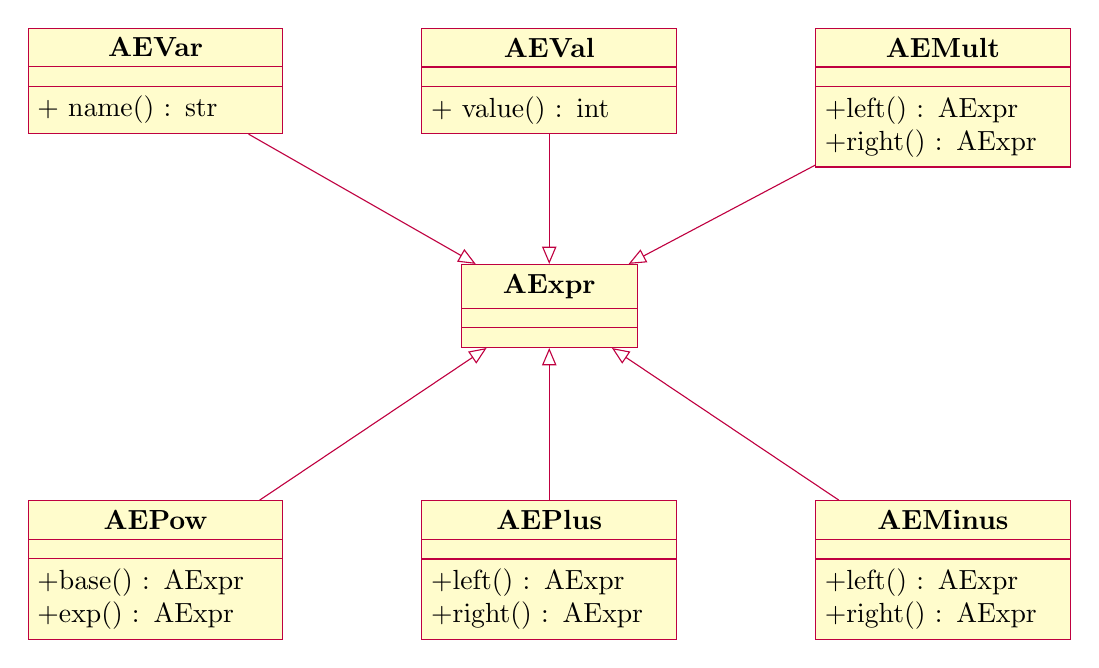
\begin{tikzpicture}
  \begin{class}[text width=2cm]{AExpr}{0,-6}
  \end{class}
  
  \begin{class}[text width=3cm]{AEVal}{0,-3}
    \inherit{AExpr}
    \operation{+ value() : int}
  \end{class}
  
  \begin{class}[text width=3cm]{AEVar}{-5,-3}
    \inherit{AExpr}
    \operation{+ name() : str}
  \end{class}
  
  \begin{class}[text width=3cm]{AEPlus}{0,-9}
    \inherit{AExpr}
    \operation{+left() : AExpr}
    \operation{+right() : AExpr}
  \end{class}
  
  \begin{class}[text width=3cm]{AEMinus}{5,-9}
    \inherit{AExpr}
    \operation{+left() : AExpr}
    \operation{+right() : AExpr}
  \end{class}

  \begin{class}[text width=3cm]{AEPow}{-5,-9}
    \inherit{AExpr}
    \operation{+base() : AExpr}
    \operation{+exp() : AExpr}
  \end{class}

  \begin{class}[text width=3cm]{AEMult}{5,-3}
    \inherit{AExpr}
    \operation{+left() : AExpr}
    \operation{+right() : AExpr}
  \end{class}
\end{tikzpicture}
\caption{Arithmetic expressions class hierarchy.}
\label{aexprs}
\end{center}
\end{figure}

In terms of usage, if we want, for instance, to represent the arithmetic expression $2 \times (x + y^2)$, we have to write the following Python code:
\begin{verbatim}
x = AEMult(AEVal(2),AEPlus(AEVar('x'),AEPow(AEvar('y'),AEVal(2))))
\end{verbatim}
The class that implements constructs related to multiplication and that used to build the above expression is derived from parent class named AExpr (which is empty and serves just the purpose of allowing to build the class hierarchy for arithmetic expressions).

\begin{lstlisting}[language=Python]
''' Parent class for remaining arithmetic expressions cases'''
class AExpr:
    pass

''' Class that represents the multiplication of two arithmetic expressions.'''
class AEMult(AExpr):


    def __init__(self,l,r):
        if not (isinstance(l,AExpr) or isinstance(r,AExpr)):
            raise AExpr_Exception
        self.__rnode   = r
        self.__lnode   = l

    def left(self):
        return self.__lnode

    def right(self):
        return self.__rnode

    def __eq__(self,other):
        match other:
            case AEMult():
                return (self.__lnode == other.left() and self.__rnode == other.right())

    def __str__(self):
        return '('+str(self.__lnode)+'*'+str(self.__rnode)+')'  
\end{lstlisting}
The code is quite compact and simple. It consists of a constructor \lstinline!__init__! that takes arguments \lstinline!l! and \lstinline!r! that refer to the left and right subexpression (that must be a particular subclass of the \lstinline!Expr! class). Both subexpressions can be accessed via the methods named \lstinline!left! and \lstinline!right!, respectively. The other methods, namely \lstinline!__eq__! and \lstinline!__str__! are responsible for comparing and pretty-printing the contents of the class, respectively.


The same type of hierarchy was implemented for Boolean expressions. In the case of specifications, those reflect the same structure of Boolean expressions, and the code is available in the file \texttt{Specs.py}. Similarly, the class hierarchy for the command's language is implemented in the file \texttt{Imp.py}. The class diagrams for each of these class hierarchies is presented, for your convenience, in the end of this document.

\subsection{The VC\_i function: reference function for completing the assignment}

We will now look into the VC\_i function, available in file \texttt{VCs.py}, and that implements the improved verification condition generation algorithm introduced in the classes. We present its Python code here to help your task of implementing the functions announced above.

First, we recall the algorithmic specification of the function:
\begin{align*}
VC(\kw{skip},Q) & ~=~ \emptyset\\
VC(x := e,Q)    & ~=~ \emptyset\\
VC(C_1;C_2,Q)   & ~=~ VC(C_1,wprec(C_2,Q)) \cup VC(C_2,Q)\\
VC(\kw{if}\,B\,\kw{then}\,C_1\,\kw{else}\,C_2,Q) & ~=~ VC(C_1,Q) \cup VC(C_2,Q)\\
VC(\kw{while}\,B\,\kw{do}\,\{I\}\,C,Q) & ~=~ \{ (I \land B) \to wprec(C,I) \} \cup VC(C,I)\\
& \:\:\:\:\:\:\:\:\:\{(I \land \neg B) \to Q\}\\
& \\
VCG(\{P\}\,C\,\{Q\}) & ~=~ \{P \to wprec(C,Q)\} \cup VC(C,Q)
\end{align*}

And now we look into the implemented code of the \textbf{VC\_i} function:
\begin{lstlisting}[language=Python,mathescape=true]
def VC_i(p,pst):
    match p:
        case Skip():
            # Case: $VC(\kw{skip},Q) = \emptyset$
            return set()
        case Assgn():
            # Case: $VC(x := e,Q) = \emptyset$
            return set()
        case Seq():
            # Case: $VC(C_1;C_2,Q) = VC(C_1,wprec(C_2,Q)) \cup VC(C_2,Q)$ 
            l = VC_i(p.left(),wprec(p.right(),pst))
            r = VC_i(p.right(),pst)
            return l.union(r)
        case IfThen():
            # Case: $VC(\kw{if}\,B\,\kw{then}\,C_1\,\kw{else}\,C_2,Q) = VC(C_1,Q) \cup VC(C_2,Q)$
            l = VC_i(p.left(),pst)
            r = VC_i(p.right(),pst)
            return l.union(r)
        case While():
            # Case: $VC(\kw{while}\,B\,\kw{do}\,\{I\}\,C,Q) = \{ (I \land B) \to wprec(C,I) \} \cup VC(C,I) \cup \{(I \land \neg B) \to Q\}$
            i = { SImp(SAnd(p.inv(),bexpr2spec(p.cond())),wprec(p.body(),p.inv())) }
            j = { SImp(SAnd(p.inv(),SNeg(bexpr2spec(p.cond()))),pst) }
            r = VC_i(p.body(),p.inv())
            return i.union(j.union(r))  
\end{lstlisting}

Note that the several lines starting with "\lstinline!# Case:!" refers to comments that we are added here (not in the original Python gile) just to make clear how the code tries to replicate what is defined at the algorithmic level of the function. This function is part of a larger function named \textbf{VCG}, thus mimicking what has been defined in the algorithmic specification. After some time looking at the produced code, it is easy to see that the function VC\_i follows exactly the structure determined in the specification, that is: it first tries to understand what kind of object is is processing (via the \lstinline!match! and \lstinline!case! constructs) and them implements the corresponding construction of sets.

\paragraph{Note on sets in Python:} In Python, mathematical sets are mapped into the primitive type of objects \lstinline!set!. Thus the usage of the \lstinline!set()! object construction to build the empty set, or the "\{ \}" notation to represent sets of objects. For more information on how to work with sets in Python, please refer to the following addresses:
\begin{itemize}
  \item W3Schools: \url{https://www.w3schools.com/python/python_sets.asp}
  \item Programiz: \url{https://www.programiz.com/python-programming/set}
  \item Real Python: \url{https://realpython.com/python-sets/}
\end{itemize}

\section{Testing your implementation}

To help on the quest for the correct implementation, the code base provided includes unit test files that will allow to check if what you have implemented is indeed according to what is expected. The files are:
\begin{itemize}
  \item \texttt{test\_Wprec.py}: this file contains unit tests that verify in the weakest precondition generation function is outputting the expected results.
  \item \texttt{test\_VCs.py}: this file contains unit tests that verify in the verification condition generation function is outputting the expected results.
  \item \texttt{test\_Z3Driver.py}: this file contains unit tests that verify in the interface with the Z3 theorem prover is outputting the expected results.
\end{itemize}

The way to use this testing scripts is straightforward, that is, if you have access to a command line, you simply run the command \lstinline!python test_Wprec.py! (and similarly with the remaining testing scripts), or you can run it directly using the "run" button available in the IDE you are using.

We now look with a bit more of detail to the structure of \texttt{test\_Wprec.py} and \texttt{test\_VCs.py}. The other unit testing file can be ignored, as it is not important for the objetives of the project (it is just there for those who want to install the Z3 theorem prover and see that the prover indeed is able to prove the correctness of the generated verification conditions generated by your implementation).

\section*{Interfacing with the Z3 theorem prover}  

As mentioned during the classes, the code that is being provided contains an interface with an external theorem prover so that we indeed can prove if programs are correct with respect to Hoare Triples. The code for this interface is available in the file \texttt{Z3Driver.py}.

To be able to use this driver, you must install the corresponding Python module. The module is named Z3Python and can be installed via the Python package manager \texttt{pip}. But you also need to install the Z3 theorem prover itself in your machine. Please follow the instructions available in the following websites:
\begin{itemize}
  \item Windows: \url{https://blog.fearcat.in/a?ID=00950-982838a1-76e1-4402-9312-d3847cb98312}
  \item Mac (using homebrew): \url{https://formulae.brew.sh/formula/z3}
  \item Linux (using Ubuntu): \url{https://www.howtoinstall.me/ubuntu/18-04/z3/} 
\end{itemize}

Note that if you are using a Linux distribution that is not Ubuntu, then you should use that distribution's own package manager (contact \url{drp@isep.ipp.pt} in case you find difficulties).



\section*{Class Diagrams for Syntax Hierarchies}

The class diagram for Boolean expressions is captured in Figure \ref{bools} by the class hierarchy presented.

\begin{figure}
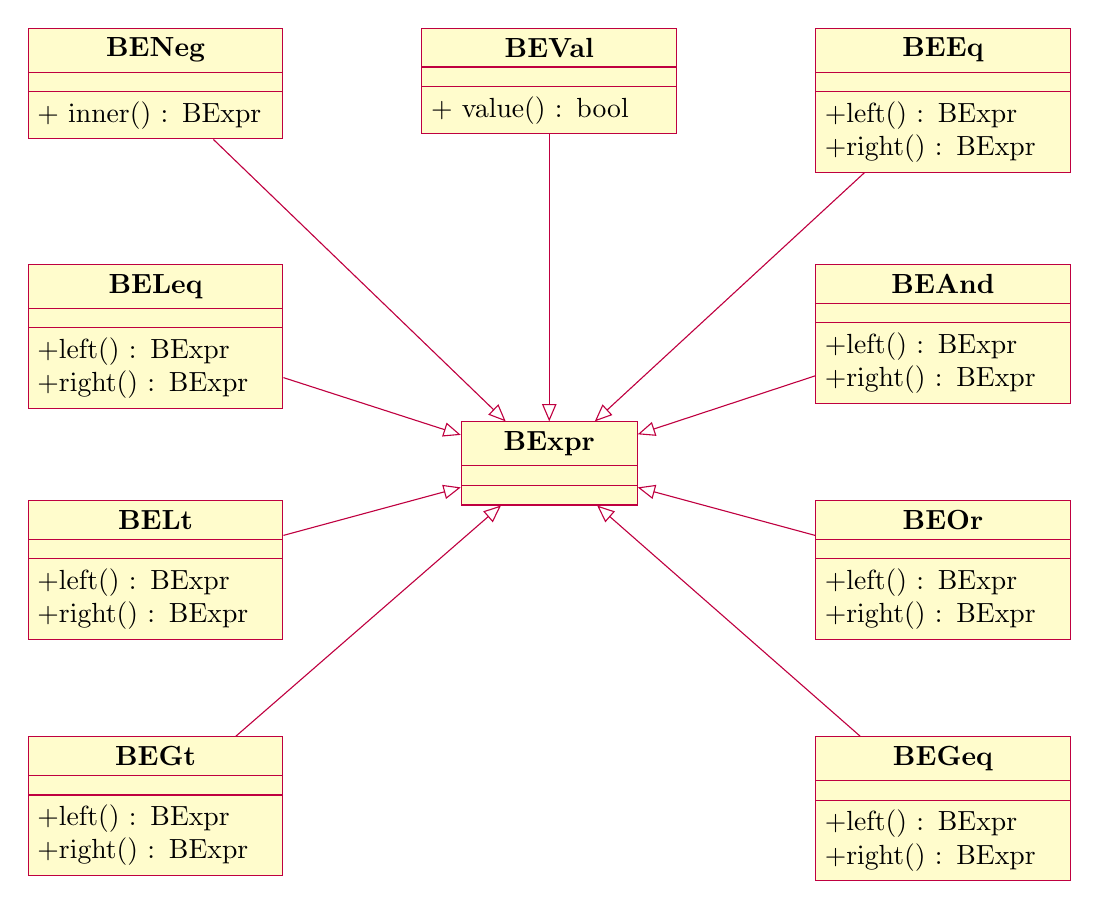
\begin{tikzpicture}
  \begin{class}[text width=2cm]{BExpr}{0,-8}
  \end{class}
  
  \begin{class}[text width=3cm]{BEVal}{0,-3}
    \inherit{BExpr}
    \operation{+ value() : bool}
  \end{class}
  
  \begin{class}[text width=3cm]{BENeg}{-5,-3}
    \inherit{BExpr}
    \operation{+ inner() : BExpr}
  \end{class}
  
  \begin{class}[text width=3cm]{BEAnd}{5,-6}
    \inherit{BExpr}
    \operation{+left() : BExpr}
    \operation{+right() : BExpr}
  \end{class}
  
  \begin{class}[text width=3cm]{BEOr}{5,-9}
    \inherit{BExpr}
    \operation{+left() : BExpr}
    \operation{+right() : BExpr}
  \end{class}

  \begin{class}[text width=3cm]{BEEq}{5,-3}
    \inherit{BExpr}
    \operation{+left() : BExpr}
    \operation{+right() : BExpr}
  \end{class}
  
  \begin{class}[text width=3cm]{BELt}{-5,-9}
    \inherit{BExpr}
    \operation{+left() : BExpr}
    \operation{+right() : BExpr}
  \end{class}

  \begin{class}[text width=3cm]{BELeq}{-5,-6}
    \inherit{BExpr}
    \operation{+left() : BExpr}
    \operation{+right() : BExpr}
  \end{class}
  
  \begin{class}[text width=3cm]{BEGt}{-5,-12}
    \inherit{BExpr}
    \operation{+left() : BExpr}
    \operation{+right() : BExpr}
  \end{class}
  
  \begin{class}[text width=3cm]{BEGeq}{5,-12}
    \inherit{BExpr}
    \operation{+left() : BExpr}
    \operation{+right() : BExpr}
  \end{class}
\end{tikzpicture}
\caption{Boolean Expressions class hierarchy.}
\label{bools}
\end{figure}

The class diagram presented in Figure \ref{specs} captures the syntax of specifications. Specifications are very similar to Boolean expressions but they also consider universal and existential quantifiers. In file \texttt{Spec.py} you can find the code that translates a Boolean expression onto a logically equivalent specification; that function is named \texttt{bexp2spec}.

\begin{figure}
\begin{center}
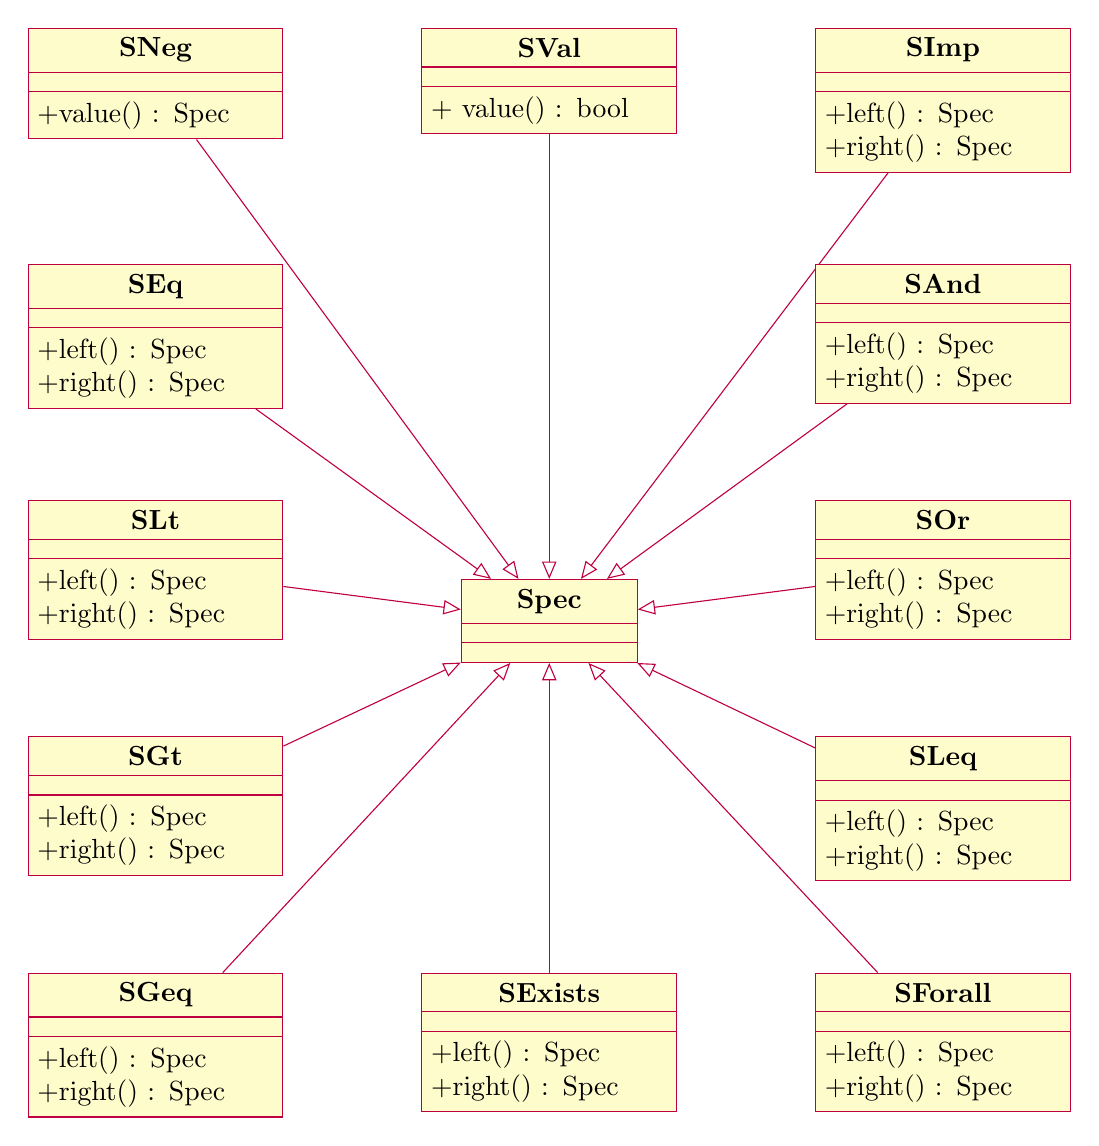
\begin{tikzpicture}
  \begin{class}[text width=2cm]{Spec}{0,-10}
  \end{class}
  
  \begin{class}[text width=3cm]{SVal}{0,-3}
    \inherit{Spec}
    \operation{+ value() : bool}
  \end{class}
  
  \begin{class}[text width=3cm]{SNeg}{-5,-3}
    \inherit{Spec}
     \operation{+value() : Spec}
  \end{class}
  
  \begin{class}[text width=3cm]{SAnd}{5,-6}
    \inherit{Spec}
    \operation{+left() : Spec}
    \operation{+right() : Spec}
  \end{class}
  
  \begin{class}[text width=3cm]{SOr}{5,-9}
    \inherit{Spec}
    \operation{+left() : Spec}
    \operation{+right() : Spec}
  \end{class}

  \begin{class}[text width=3cm]{SImp}{5,-3}
    \inherit{Spec}
    \operation{+left() : Spec}
    \operation{+right() : Spec}
  \end{class}
  
    \begin{class}[text width=3cm]{SEq}{-5,-6}
    \inherit{Spec}
    \operation{+left() : Spec}
    \operation{+right() : Spec}
  \end{class}
  
      \begin{class}[text width=3cm]{SLt}{-5,-9}
    \inherit{Spec}
    \operation{+left() : Spec}
    \operation{+right() : Spec}
  \end{class}
  
     \begin{class}[text width=3cm]{SGt}{-5,-12}
    \inherit{Spec}
    \operation{+left() : Spec}
    \operation{+right() : Spec}
  \end{class}
  
      \begin{class}[text width=3cm]{SLeq}{5,-12}
    \inherit{Spec}
    \operation{+left() : Spec}
    \operation{+right() : Spec}
  \end{class}
  
      \begin{class}[text width=3cm]{SGeq}{-5,-15}
    \inherit{Spec}
    \operation{+left() : Spec}
    \operation{+right() : Spec}
  \end{class}
  
      \begin{class}[text width=3cm]{SForall}{5,-15}
    \inherit{Spec}
    \operation{+left() : Spec}
    \operation{+right() : Spec}
  \end{class}

      \begin{class}[text width=3cm]{SExists}{0,-15}
    \inherit{Spec}
    \operation{+left() : Spec}
    \operation{+right() : Spec}
  \end{class}
  
\end{tikzpicture}
\end{center}
\caption{Specifications class hierarchy.}
\label{specs}
\end{figure}




\end{document}